% TODO: Pictures

\documentclass[12pt, a4paper]{article}

\usepackage{preamble}

% TODO: Decide who focuses on which parts. There will of course be overlap and
% we will all review and discuss the different sections.

\title{Models of Associative Memory}

\author{Wenting Jin, Lucas Arnström \& Robin Eklind}

\begin{document}

\maketitle

\tableofcontents

\clearpage

% TODO: Add abstract?

% === [ Introduction ] =========================================================

\section{Introduction}

\subsection{Associative Memory}

Definition of associative memory.

Distinction between auto-associative and hetero-associative memory.

% === [ Models of Associative Memory ] =========================================

\section{Models of Associative Memory}

\subsection{Hopfield Networks}

% Wenting.
Hopfield's model is an associative(content-addressable) memory model with threshold and feedback.

In paper from J.J.Hopfield(1982) \cite{computational_abilities}, the drawbacks of Perceptron were addressed through its intractable back-coupling, lack of abstraction properties and requirement of synchronism. Information storage was improved with help of Nonlinearity, and emergent computational properties were obtained from simple properties of many cells rather than complex circuitry(which is a result of linear associativity). The input-output relationship of nonlinear computation, binary threshold units and concept of the energy function were introduced.

Collective behaviors of the model was studied and resulted with the following findings: a few stable states was resulted from most of the initial state space, properties necessary for a physical content-addressable memory were not dependent on the symmetry of the connectivity matrix $T_{ij}$. Statement supported by findings from experiments is that "about 0.15N(memory storage bits, number of neurons) states can be simultaneously remembered before error in recall is severe", which refers to the memory capacity of the associative memory. Case with arbitrary starting state was studied and results of memories near to the starting state was highly produced. The nominally assigned memories which were called "attractors" dominates the phase flow whereas the flow is not entirely deterministic, which leads to a convergence to local optimum.

Case of consistent internal correlations in the memory was as well addressed, and Hebb synapses was used and slightly modified to generate nonsymmetric term~$\delta T_{ij}$, which limitation of sequence of four states was addressed.



\subsubsection{Implementation Example: Optical Information Processing}
In paper from D.Psaltis and N.Farhat(1985) \cite{optical_processing}, thresholding and feedback properties from Hopfield model was used in implementation of an optical system that processes optical information.

Enhanced error-correcting capability is one important outcome which is benefited from Nonlinearity of Hopfield model. With $M$ words of each binary vector $v_i$ with length of N bits, matrix $T_{ij}$ represents a storage of information. Matrix $T_{ij}$ gets multiplied by a stored binary vector $v'_i$ results in a \texttt{pseudoeigensystem} if $N$ is sufficiently larger than $M$. This indicated that the output vector $v''_i$ equals the input.

Supposed nonlinear iterative procedural experiments of certain number of known bits $N_1$ and the rest bits set to zero inside total of $N$ bits long vector were addressed to discover under what conditions the number of correct bits $N_2$ in output will be higher than $N_1$. A SNR(signal-to-noise ratio) equation which consists ratio of the expected value to the standard deviation on the same output vector, was used. As the Hopfield model has studied on the convergence property with respect to asynchronous operations, insensitivity to imperfections(nonuniformities, exact form of the threshold operation and errors in $T_{ij}$ matrix) and correct convergence obtained with thresholded $T_{ij}$. These all become most desired properties in optical implementation. Detailed optical implementation with 2D inputs was presented which was based on spatial-frequency multiplexing. Methods using Fourier transform, transmitting amplitude(weighted sum) and integral of the product of the input images were introduced in such an implementation. The robustness of a such system with nonlinear feedback becomes the most important feature.
As a conclusion, the implementation with the capabilities and limitations of optical techniques matches excellently with the Hopfield model that requires global, linear operations and local, point nonlinearities in a fully interconnected optical system.



\subsubsection{Memory Capacity with Modification: \\ replacing sigmoid neuron with a nonmonotonic neuron}
In paper from S.Yoshizawa, M.Morita and S.Amari(1992) \cite{capacity_of_nonmonotonic_model} it started with introduction of a new method by replacing sigmoid neuron with a nonmonotonic neuron and discussed theorectically on potential of absolute capacity(the maximum number of randomly generated patterns which are memorized as the equilibria of the network with the correlation-type connection weights) to be of order $n$ (nearly equal to 0.4n).

Previous memory capacities were briefly introduced that Hopfield(1982) model's associative memory capacity is 0.15n, the proven result of absolute capacity is asymptotically $ \frac{n}{2\log{n}} $ from McEliece, Posner, Rodemich, \& Venkatesh, 1987; Weisbuch, 1985), and relative capacity(recalling process) is about 0.14n(with admission of small percent of errors) with replica method but about 0.16n with a simply approximation method from respectively two different research work.

Various research suggestions were mentioned though all failed to deal completely with flaws of the conventional model, that both absolute and relative capacities are too small as well as the existence of large number of spurious memories. With a nonmonotonic neuron the result turned to be 0.4n for the absolute capacity which is even greater than relative capacity while the spurious memory disappeared.

With conventional neuron, memorized pattern is unstable ,whereas a basin of attraction around memorized pattern was shown with nonmonotonic neuron by replacing sigmoid function with a nonmonotonic output function \ref{fig:nonmonotonic} to neuron elements from the recalling process of an autocorrelation associative memory. This was named as Morita Model in the paper though it is essentially an extension from Hopfield Model.
With by then the existence of equilibrium solutions and local stability, the authors did not further investigate on problems as the following: the size of the basin of attraction, the full sketch of spurious memories and the behaviour for clustered memorized patterns, which leaves more research work for future researchers to understand better associative memory with nonmonotonic neurons.


\begin{figure}[h!]
\centering
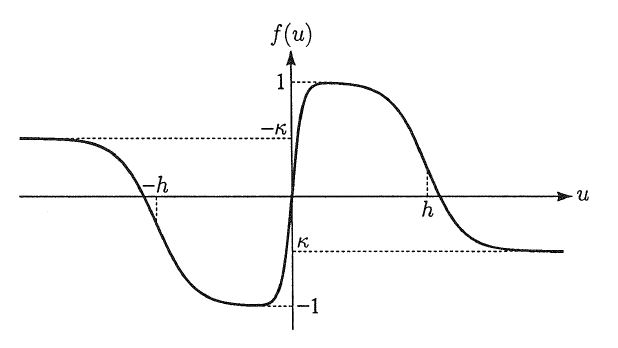
\includegraphics[scale = 0.8]{nonmonotonic.JPG}
\caption{The nonmonotonic output function, S.Yoshizawa, M.Morita and S.Amari(1992)}
\label{fig:nonmonotonic}
\end{figure}



%THIS IS STH EXTRA OUTSIDE HOPFIELD
\subsection{Experiment on Implicit Memory for Novel Associations between pictures: \\ Effects of Stimulus Unitization and Aging\cite{stimulus_unitization_and_aging}}

From various previous research, concepts such as associative priming, unitization, difference between conceptual and perceptual associative priming, verbal versus pictorial material/stimuli and roll of spatial proximity were briefly summarized.


Experiments with pictorial stimuli(paired pictures) were done in 3 consecutive stages, where the result from first stage showed no evidence on requirement of spatial contiguity, though associative priming was enhanced compared to with spatially separated stimuli, which proved "implicit memory for novel associations still can occur in the absence of an emergent conceptual representation". The second experiment was an extension from the first experiment, with focus on the effects of aging and spatial contiguity of the same topic of stimuli on novel association priming between pictures, where stunning result was shown that "associative priming is age invariant"(exposure of pictures was longer with older group to yield a matched performance in the baseline). The last experiment was based on both first and second experiments that "associative priming with pictorial stimuli is modulated by spatial contiguity but not by aging", and the study proved further evidence for the notion that novel association priming for picture pairs is mediated by the PRS(Perceptual Representation System).


% Mostly auto-associative. Also hetero-associative?

\subsection{Bidirectional Associative Memory}

Mostly hetero-associative. Also auto-associative.

\subsection{Boltzmann Machine}

% --- Lucas

\begin{figure}[htbp]
	\begin{center}
		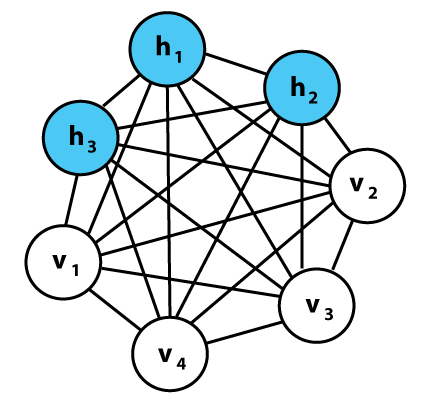
\includegraphics[width=0.5\textwidth]{inc/boltzmann_machine.png}
		\caption{Illustration of a Boltzmann Machine. The blue units represents three hidden units, while the four white units represents four visible units.\protect\footnotemark}
		\label{fig:boltzmann_machine}
	\end{center}
\end{figure}
\footnotetext{Original image (CC BY-SA): \url{https://en.wikipedia.org/wiki/File:Boltzmannexamplev1.png}}

The "Boltzmann Machine" (BM) is a form of "parallel constraint satisfaction network" \cite{ackley1985learning}. It is capable of learning the underlying constraints of a domain by only being shown examples of it. The BM is composed of units forming a complete graph where the connection between two units are symmetric, meaning that the weight on the connection is the same in either direction. No unit has a connection to itself. The units are binary, meaning that they can assume one of two states, on or off. The state of a unit is determined by a probabilistic function based on the states of the units neighbours. A strong connection (high weight value) between two units indicates that if either of these two units are active, the other one should probably be active as well. While a weak connection (low weight value) indicates that these should probably not be active at the same time.

The BM is notably similar to the Hopfield network in that it also defines a global energy state of the system, utilizing the same equation that determines the global energy value. Each global state can be identified by the energy of the system in that state. By forcing the values of the visible units to represent a training set the system attempts to find an energy configuration that is compatible with the given input. The resulting energy state can then be interpreted as to how well the given data fulfills the constraints of the domain. Thus by minimizing the energy the system learns an interpretation of the problem that increasingly satisfies the constraints of the domain.

The simplest way to minimize the energy into a local minimum of the system is to change each unit into a value that results in a lower energy state. The data needed to determine this change is locally accessible to each unit. If the sum of all values for a given units neighbour exceeds the threshold of that unit, the resulting state of the unit should be on. Otherwise it should be off. This is the usual algorithm for binary units.

Because of this deterministic algorithm it suffers from the usual weaknesses of gradient descent algorithms, namely it gets stuck in local minima if its initial state is close to one. In order to alleviate the algorithm of this problem noise is introduced in the training. This allows the network to "jump" out of these minima into configurations of higher energy. The algorithm used for noise introduction is a variation of the "Metropolis algorithm" \cite{metropolis1953equation} that was used to study thermodynamic systems. This modified version introduces a concept of temperature to the machine. The machine then tries to reach "thermal equilibrium" during training. Meaning that the machine is allowed to run repeatedly until the global energy of the system converges to a fixed state over a temperature that is initially high and then slowly decreased over the runtime of the system. The probability of finding the system in a global state after it has reached thermal equilibrium follows a Boltzmann distribution.

%TODO write more about this temperature thing
%TODO write more about the probabilistic features of the BM as well as the boltzmann distribution that gives the system its name.

Training is conducted in two phases, the first is called the "positive" phase were the visible units of the machine are set to the values of the training set. The next phase is called the "negative" phase. During this phase the machine is allowed to run freely, independent of the training set. The machine is iteratively switched between these two phases for the duration of the training until it reaches thermal equilibrium. The goal of the training is for the machine to generate the input vector with a high probability.

% --- NOTES
%The difference between the BM and the Hopfield network is mainly that the nodes (or units as they are referred to in the original paper) of the Boltzmann Machine are stochastic by nature.
%The BM can be used for constraint satisfaction problems that involve a large amount of weak constraints.



%\subsection{Hamming networks}

%foo

% TODO: Decide whether to include Hamming networks or not.

\subsection{Memory Resistor}

%Robin.

Memory resistors, memsistors for short, are passive circuits which change their resistance as current flows through them, and maintain their resistance in between use. In other words, memsistors remember past flows of current (i.e. store state), and control resistance based on this knowledge (i.e. stored state). Several similarities have been identified bewteen the properties of memsistors and synapses, which make them interesting candidates for associative memory models.

TODO: Extend. Artificial synapses experiment using memsistors conducted in 2010, empiricially validating the formation of associative memories using three neurons and two synapses \cite{memristor_conditioning}.

TODO: Extend. The memsistor was hyphosized in 1972 by Leon Chua, the father of non-linear curcuit theory, who presented it as the missing fundamental cirtuit element (see figure \ref{fig:circuit_elements}) \cite{chua_memristor}. Looking at the current~$I$ and voltage~$V$ plot, a memsistor may be identified by the pinched hysteresis loop going through origo (see figure \ref{fig:pinched_hysteresis}. TODO: Explain the underlying reason of the hysteresis loop, i.e. alterating between two states (metastable switch).

\begin{figure}[htbp]
	\begin{center}
		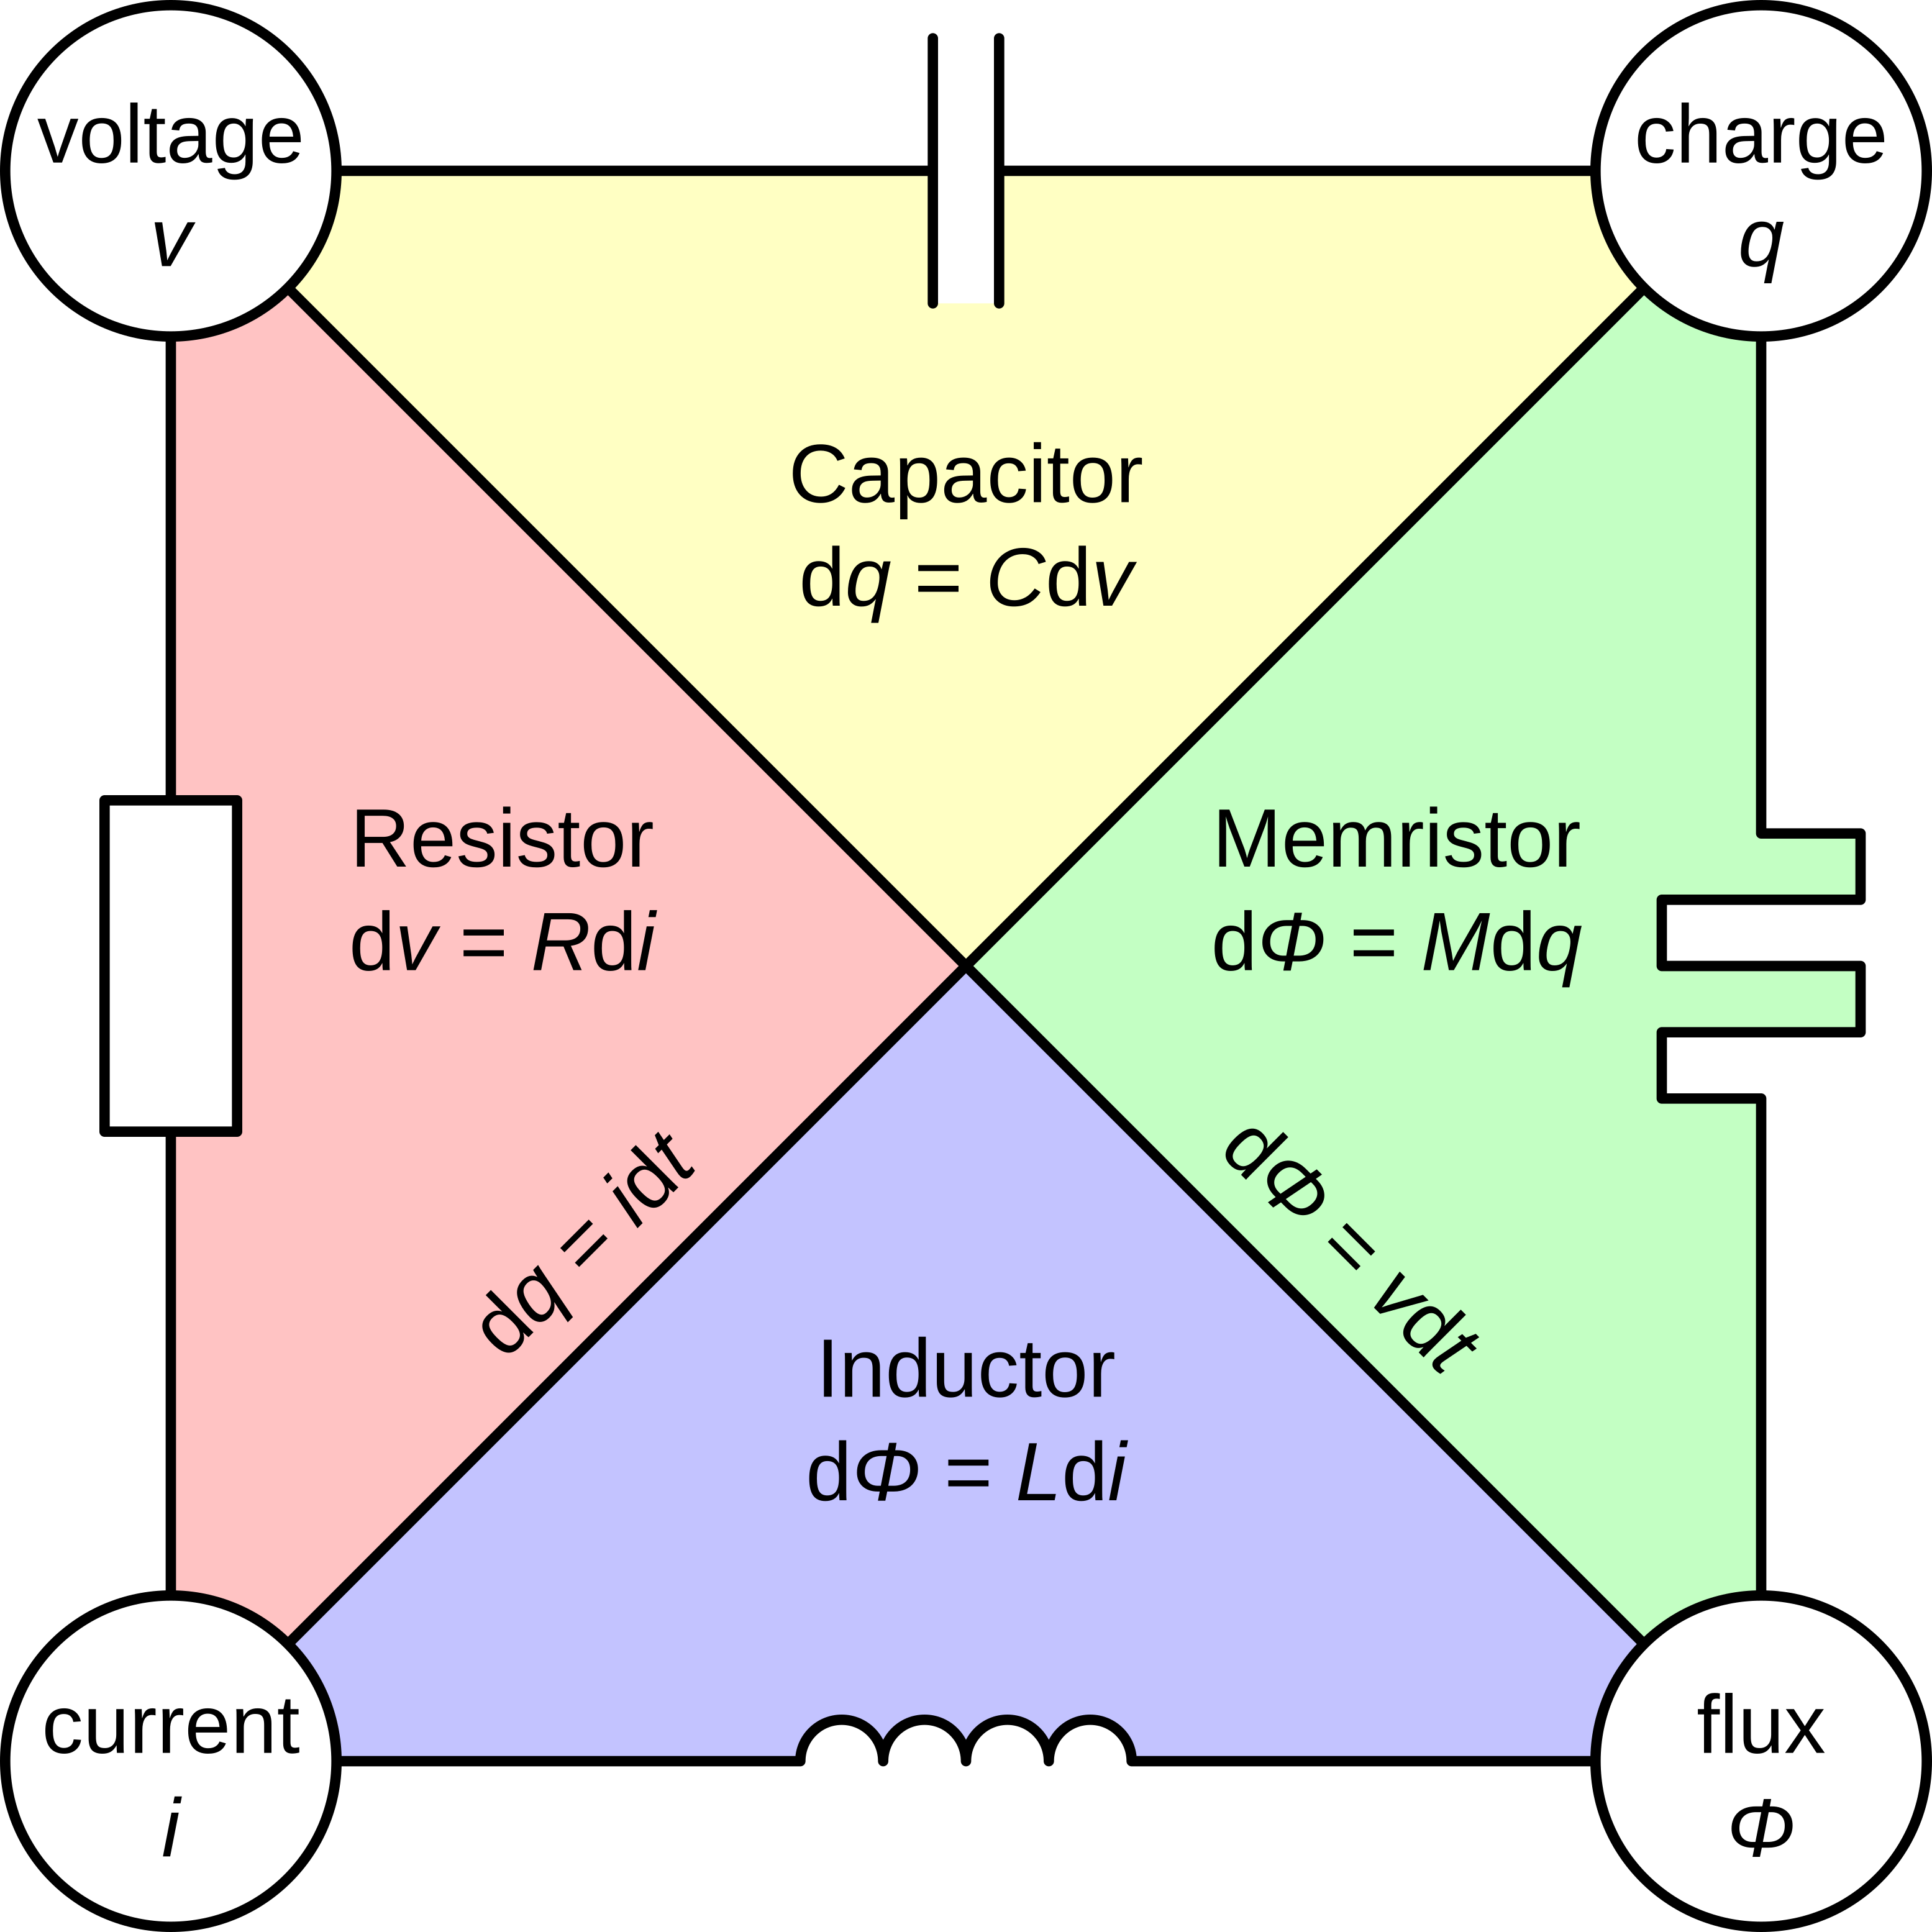
\includegraphics[width=0.5\textwidth]{inc/circuit_elements.png}
		\caption{Fundamental circuit elements.\protect\footnotemark}
		\label{fig:circuit_elements}
	\end{center}
\end{figure}
\footnotetext{Original image (CC BY-SA): \url{https://en.wikipedia.org/wiki/File:Two-terminal_non-linear_circuit_elements.svg}}

\begin{figure}[htbp]
	\begin{center}
		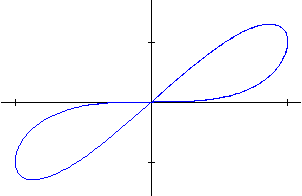
\includegraphics[width=0.5\textwidth]{inc/pinched_hysteresis.png}
		\caption{A pinched hysteresis loop plotted on an IV-curve.\protect\footnotemark}
		\label{fig:pinched_hysteresis}
	\end{center}
\end{figure}
\footnotetext{Original image (CC BY-SA): \url{https://en.wikipedia.org/wiki/File:Pinched_crossing_hysteresis.png}}

TODO: Extend. In 2008, HP released a paper titled \textit{The missing memristor found}, which outlined the hardware implementation of a memsistor \cite{hp_memristor_found}, thus validating the existence of the hypothesized memsistors circuit element. Retrospectively, several research groups had discovered circuits with the tell-tale properties of memsistor, i.e. with a pinched hysteresis loop. TODO: Include ref about prior research, before 2008.

% === [ Current Capabilities ] =================================================

\section{Current Capabilities}

Definitions of capacity.

\begin{itemize}
\item Absolute capacity.
\item Relative capacity.
\item Capacity of associative memory
\item Relative capacity of recalling process
\end{itemize}

\subsection{Hopfield Network}

%Wenting.

1982, $0.15n$ (capacity of associative memory)

% Above 0.15n releases the constraint on symmetries according to Olle.

1985, proven $ \frac{n}{2\log{n}} $ (absolute capacity)

1985, $0.14n$ (relative capacity of recalling process)

1993, $ n ~= 0.4n $ (new result, absolute capacity)

\subsection{Bidirection Associative Memory}

% TODO: Check.

foo

\subsection{Boltzmann Machine}

%Lucas.

Unfortunately, the Boltzmann Machine can only be used for simpler problem domains. If the BM is scaled beyond any trivial domain it becomes too slow and almost stops learning. This is due to the fact that all units of the BM are fully connected to each other which does not scale well.

In order to use the BM for bigger tasks a restriction has to be made. Namely, connections between units in the same layer can not be allowed. This is called the Restricted Boltzmann Machine (or "Harmonium" as the original author referred to it) \cite{smolensky1986information}.

Versions of the Restricted Boltzmann Machine (RBM) have been successfully used in deep learning \cite{hinton2012better} and speech recognition \cite{dahl2010phone}.

The general idea when using RBM's in deep learning is to "stack" several RBM's on top of each other. The activities of the units in the hidden layer of one RBM can be used as input vector for an other RBM. This way the overall system does not have the problem with scalability that the ordinary Boltzmann Machine suffered. Every time a new layer is added on top the generative model is improved.

\subsection{Memory Resistor}

%Robin.

Proof of concept in 2010, using 3 neurons and 2 synapses to achieve 1 associative memory formation.

% === [ Future Potential ] =====================================================

\section{Future Potential}

\subsection{Intelligent Systems}

Intelligence defined by ability to make predictions, not behaviour \cite{intelligence_is_prediction}.

\subsection{Energy Efficiency}

Network in its true sense, \textit{the net is doing all the work} \cite{net_doing_all_the_work}.

\cite{ahah}

%Current computer architectures are designed around major bottlenecks, huge amounts of data has to be shuffled back and forth to perform computations. Reaching its limits; transistors now so small that they only allow a single electron to pass through (similar in size to the ion channels). At this scale, problems arise when transistors may allow electrons to pass through, when they shouldn't and wise versa; which leads to unpredictable behaviour (small bursts of ones when should be be all zero, and wise versa.)

%The brain, parallel, error correcting, memory efficient. (not doing a lot of unnecessary data shuffling?)

% === [ Conclusion ] ===========================================================

\section{Conclusion}

foo

% === [ Research Literature ] ==================================================

Preliminary list of references, cited to force inclusion within the bibliography.

% TODO: Add to this list throughout the project.

% Wenting
\cite{computational_abilities} \cite{optical_processing} \cite{capacity_of_nonmonotonic_model} \cite{stimulus_unitization_and_aging}

% Lucas
%\cite{ackley1985learning} \cite{capacity_of_hopfield} \cite{high-order_neural_networks} \cite{neural_network_models_for_associative_memory} \cite{sparsely_encoded_associative_memory}

% Robin
\cite{memsistor} \cite{principle_of_neural_associative_memory} \cite{parallel_models_of_associative_memory} \cite{associative_memory_using_small-world_architecture} \cite{associatron} \cite{associative_search_network} \cite{deep_machine_learning} \cite{on_associative_memory} \cite{from_cell_to_cortex} \cite{ahah}

\bibliography{references}

\end{document}
